\chapter{Implementation}
\label{cha:Implementation}

This chapter presents the app's software basics with a focus on the \ac{UI} framework and data persistence.
It also outlines the implementation of geofencing and reminder behavior, concluding with a test feature designed to make the app more user-friendly.

\section{Software Basics}
The app is built using iOS technologies.
SwiftUI was chosen as the framework for building the \acs{UI}, while SwiftData is used for managing and persisting data across app sessions.

\subsection{SwiftUI}
SwiftUI is Apple's declarative \acs{UI} framework, introduced in 2019, which allows developers to create user interfaces with less boilerplate code compared to UIKit.
One of the advantages of SwiftUI is that \acs{UI} updates occur automatically when the underlying data changes, instead of using view controllers and manual \acs{UI} updates.
This makes the framework particularly powerful when combined with SwiftData as the \acs{UI} can react dynamically to stored data.

\subsection{SwiftData}
SwiftData simplifies data storage and retrieval in Swift applications, allowing developers to define models directly in Swift using macros instead of external files like Core Data. 
A \lstinline{ModelContainer} manages persistence, determining whether data is stored locally or in iCloud. 
Within the app, it acts as a central storage hub for all models.
To enable persistence for a specific model, the container is initialized as shown in Program \ref{prog:modelcontainer}.

\begin{program}
    \begin{SwiftCode}
    let modelContainer: ModelContainer = ModelContainer(for: Reminder.self)\end{SwiftCode}
    \caption{Initializing the \lstinline{ModelContainer} for SwiftData persistence}
    \label{prog:modelcontainer}
\end{program}

The \lstinline{ModelContainer} stores the data models, but the actual operations such as inserting and deleting data are performed using a \lstinline{ModelContext}. 
The \lstinline{ModelContext} serves as the interface between the app's logic and the database, allowing modifications to stored data during runtime.
Marking a class with the \lstinline{@Model} macro signals to SwiftData that it should be persistently stored. 
At compile time, Swift automatically generates a schema and essential methods for managing data without adding runtime overhead.
To fetch and track changes in stored data, the \lstinline{@Query} macro can be used alongside \lstinline{@Model}.
It automatically retrieves data from the \lstinline{ModelContainer} and updates the \acs{UI} whenever changes occur without manual database queries.
In the app, \lstinline{ModelContext} is set as an environment value, and \lstinline{@Query} dynamically accesses the array of reminder objects as illustrated in Program \ref{prog:modelcontext}, which demonstrates deleting and inserting a reminder into the database.

\begin{program}[htbp]
    \begin{SwiftCode}
    @Environment(\.modelContext) private var modelContext
    @Query var reminders: [Reminder]
    ...
    modelContext.delete(reminders[index])
    modelcontext.insert(reminder)\end{SwiftCode}
    \caption{Using \lstinline{ModelContext} for modifying persistent data and \lstinline{@Query} for fetching data}
    \label{prog:modelcontext}
\end{program}

In addition to data persistence with SwiftData, the app also incorporates \lstinline{AppStorage} for lightweight preference storage. 
\lstinline{@AppStorage} is a SwiftUI property wrapper built on top of \lstinline{UserDefaults} and is commonly used for saving app settings or user preferences to persist across app launches and any updates trigger a \acs{UI} refresh, ensuring the latest data is always displayed.

\begin{program}[htbp]
    \begin{SwiftCode}
    @AppStorage("ReminderMode") static var reminderMode: ReminderMode = .distance
    @AppStorage("TimeInterval") static var timeInterval: TimeInterval = ._7min
    @AppStorage("StationInterval") static var stationInterval: StationInterval = ._4stations
    @AppStorage("DistanceInterval") static var distanceInterval: DistanceInterval = ._1km
    @AppStorage("Vibration") static var vibration: Bool = true
    @AppStorage("Alarm") static var alarm: Bool = true\end{SwiftCode}
    \caption{Using \lstinline{@AppStorage} to persist user preferences in the app}
    \label{prog:appstorage}
\end{program}

\section{User Interface}
The app's \ac{UI} consists of three main views, accessible via a tab bar at the bottom.
In addition to these primary views, the app includes several secondary views.
Figure \ref{fig:viewstructure} presents a diagram illustrating the hierarchical structure of these views within the app. 
The following sections provide an overview of each view and explain the user journey through the application.

\begin{figure}[htbp]
    \centering
    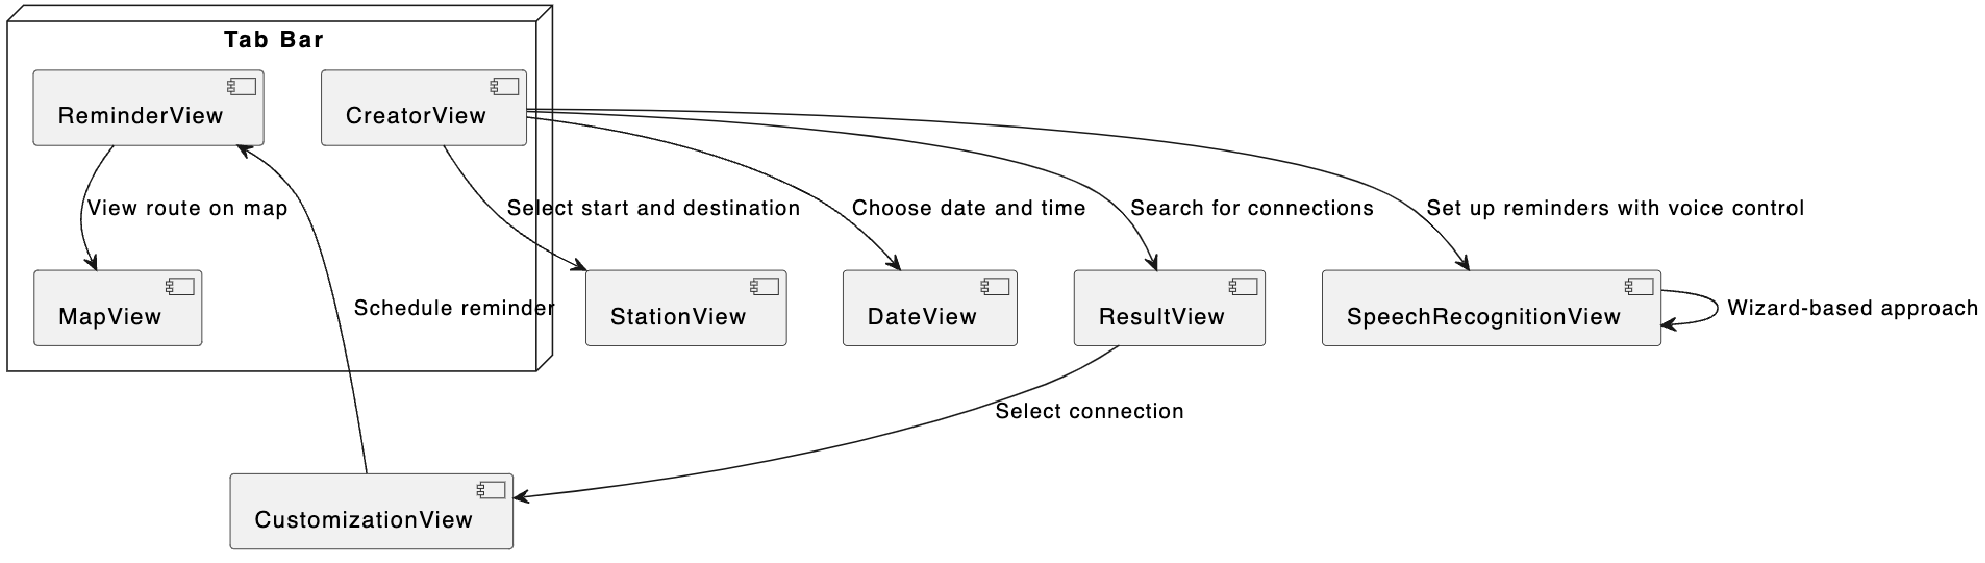
\includegraphics[width=1\textwidth]{ViewStructure.pdf}
    \caption{Diagram illustrating the hierarchical structure of main and secondary views}
    \label{fig:viewstructure}
\end{figure}

\subsection{CreatorView}
As introduced in Chapter \ref{cha:Concept}, the \lstinline{CreatorView} serves as the app's entry point, guiding users through the trip planning process. 
This view is illustrated in Figure \ref{fig:creatorview} (a), where users can select their start location \circnum{1} and destination \circnum{2} by tapping the corresponding buttons.
This action opens \lstinline{StationView} in a sheet from the bottom, where users can search for a station and select it as seen in Figure \ref{fig:creatorview} (b). 
Once a station is chosen, its name replaces the button label.
Below the station selection, the interface provides a date and time selector \circnum{3} which defaults to immediate departure. 
Tapping it opens \lstinline{DateView} in a sheet as depicted in Figure \ref{fig:creatorview} (c), where users can choose between departure or arrival time \circnum{6} and set the date \circnum{7} and time \circnum{8}.
Additionally, a microphone icon button \circnum{4} in Figure \ref{fig:creatorview} (a) provides access to the \lstinline{SpeechRecognitionView}, which offers a wizard-based approach for setting up reminders through AI-assisted voice processing. 
This test feature is discussed in detail in Subsection \ref{sec:speechview}.

The search button \circnum{5} in Figure \ref{fig:creatorview} (a) allows users to retrieve simulated public transport connections based on the selected parameters. 
Upon pressing the button, the app navigates to the \lstinline{ResultView} in Figure \ref{fig:customizationview} (a), which displays details such as departure and arrival times, station names and line ID as seen in \circnum{9}. 
Since no suitable open \acs{API} for public transport data could be found, the displayed connections are simulated.
Each entry includes a plus button \circnum{10} and pressing this button signals the app to navigate to the \lstinline{CustomizationView}, where users can configure their reminder preferences. 
As depicted in Figure \ref{fig:customizationview} (b), this view provides options to select a reminder mode \circnum{11} and set the corresponding interval \circnum{12}. 
Users can also choose additional alert settings, such as vibration \circnum{13} and an audible alarm \circnum{14}. 
When enabled, these alerts are scheduled to occur at a predefined interval.
These preferences are stored, ensuring they are pre-filled when the \lstinline{CustomizationView} is accessed again. 
Pressing the 'Schedule Alert' button \circnum{15} schedules the notification, vibration and alarm. 
The app then transitions to the \lstinline{ReminderView}, which is described in the following section.

\begin{figure}[H]%
    \centering
    \subfloat[\centering]{{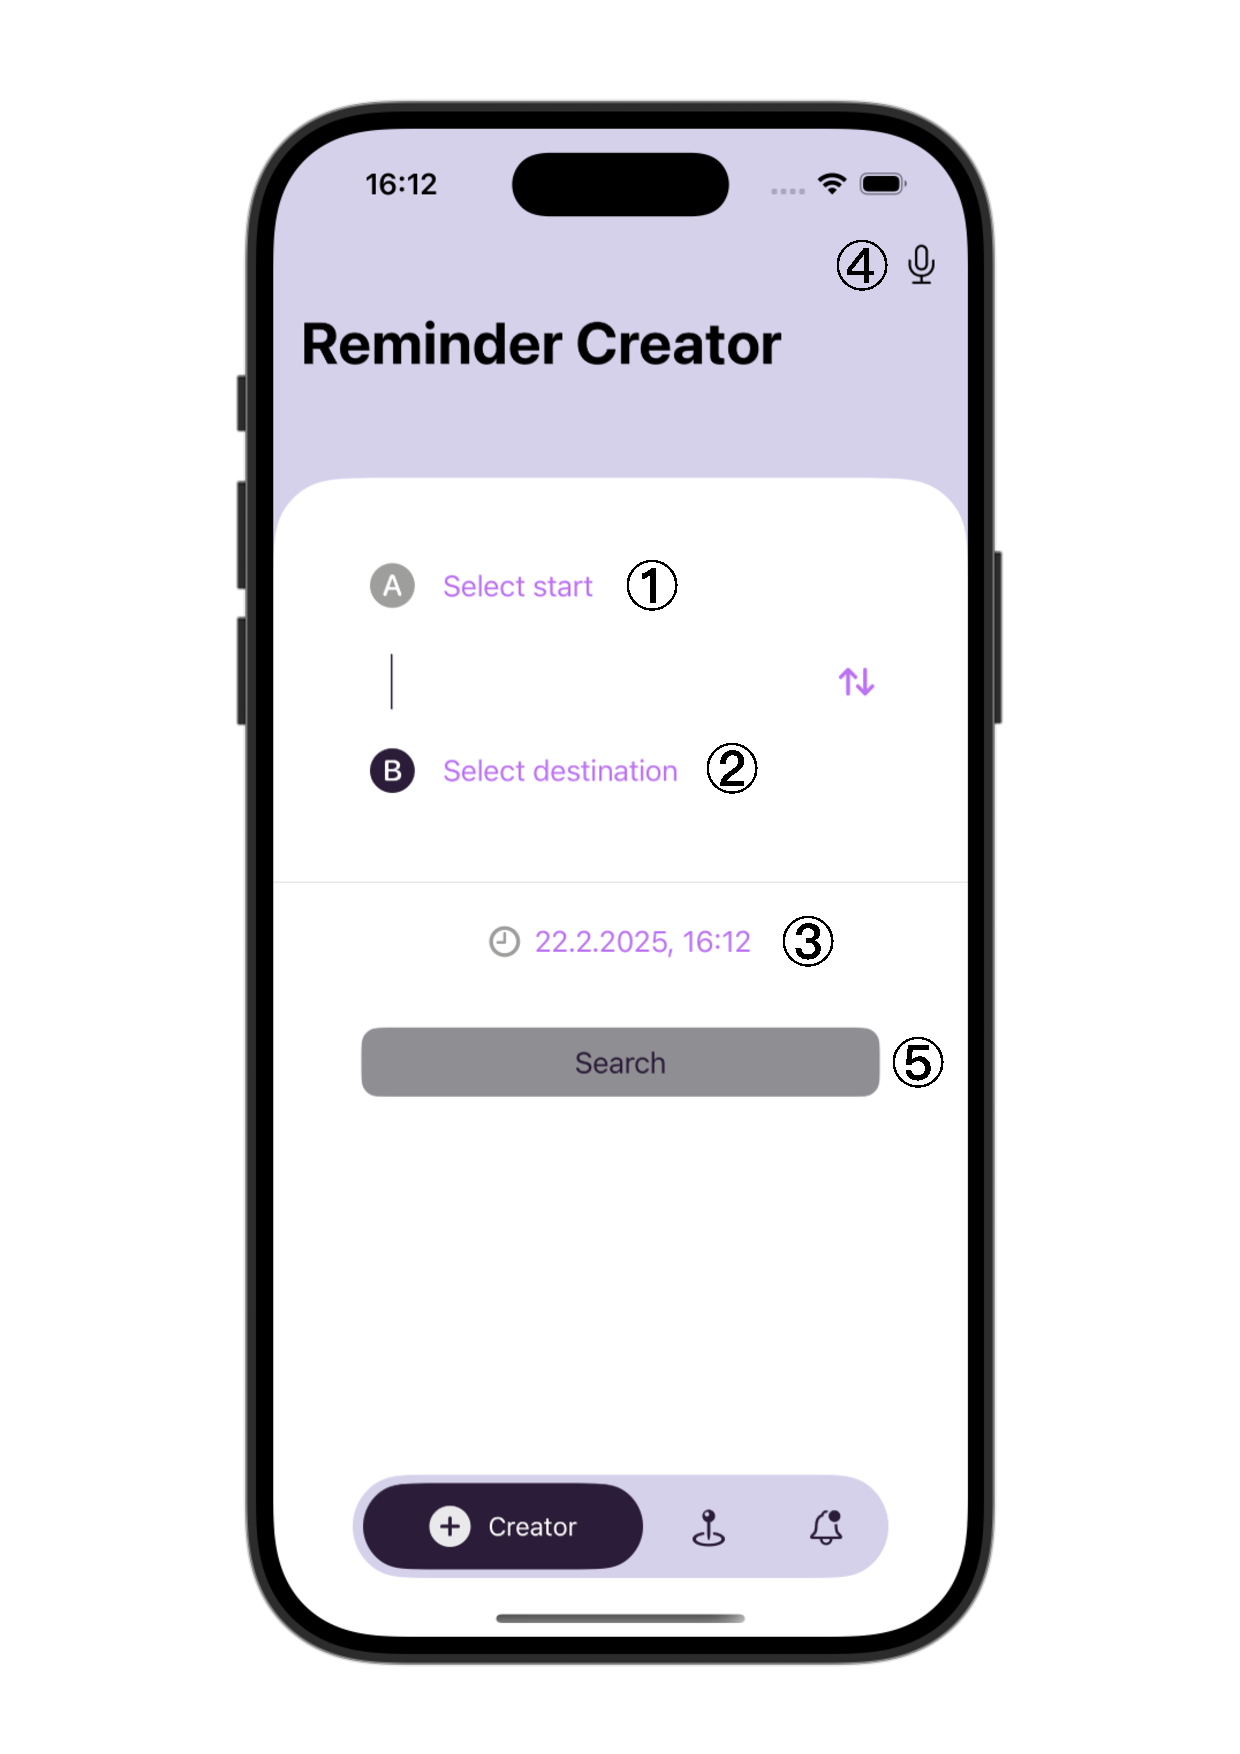
\includegraphics[width=4cm]{CreatorView.pdf}}}%
    \qquad
    \subfloat[\centering]{{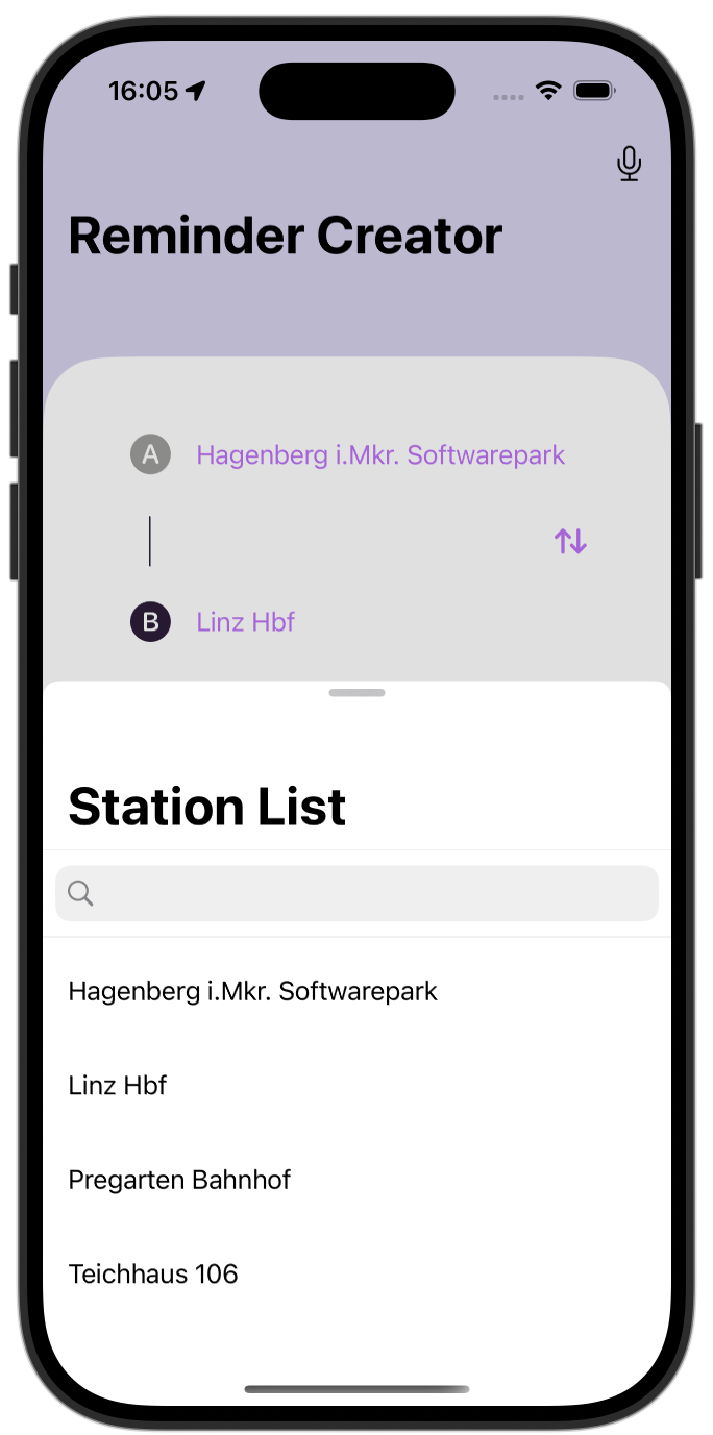
\includegraphics[width=4cm]{CreatorView2.pdf}}}%
    \qquad
    \subfloat[\centering]{{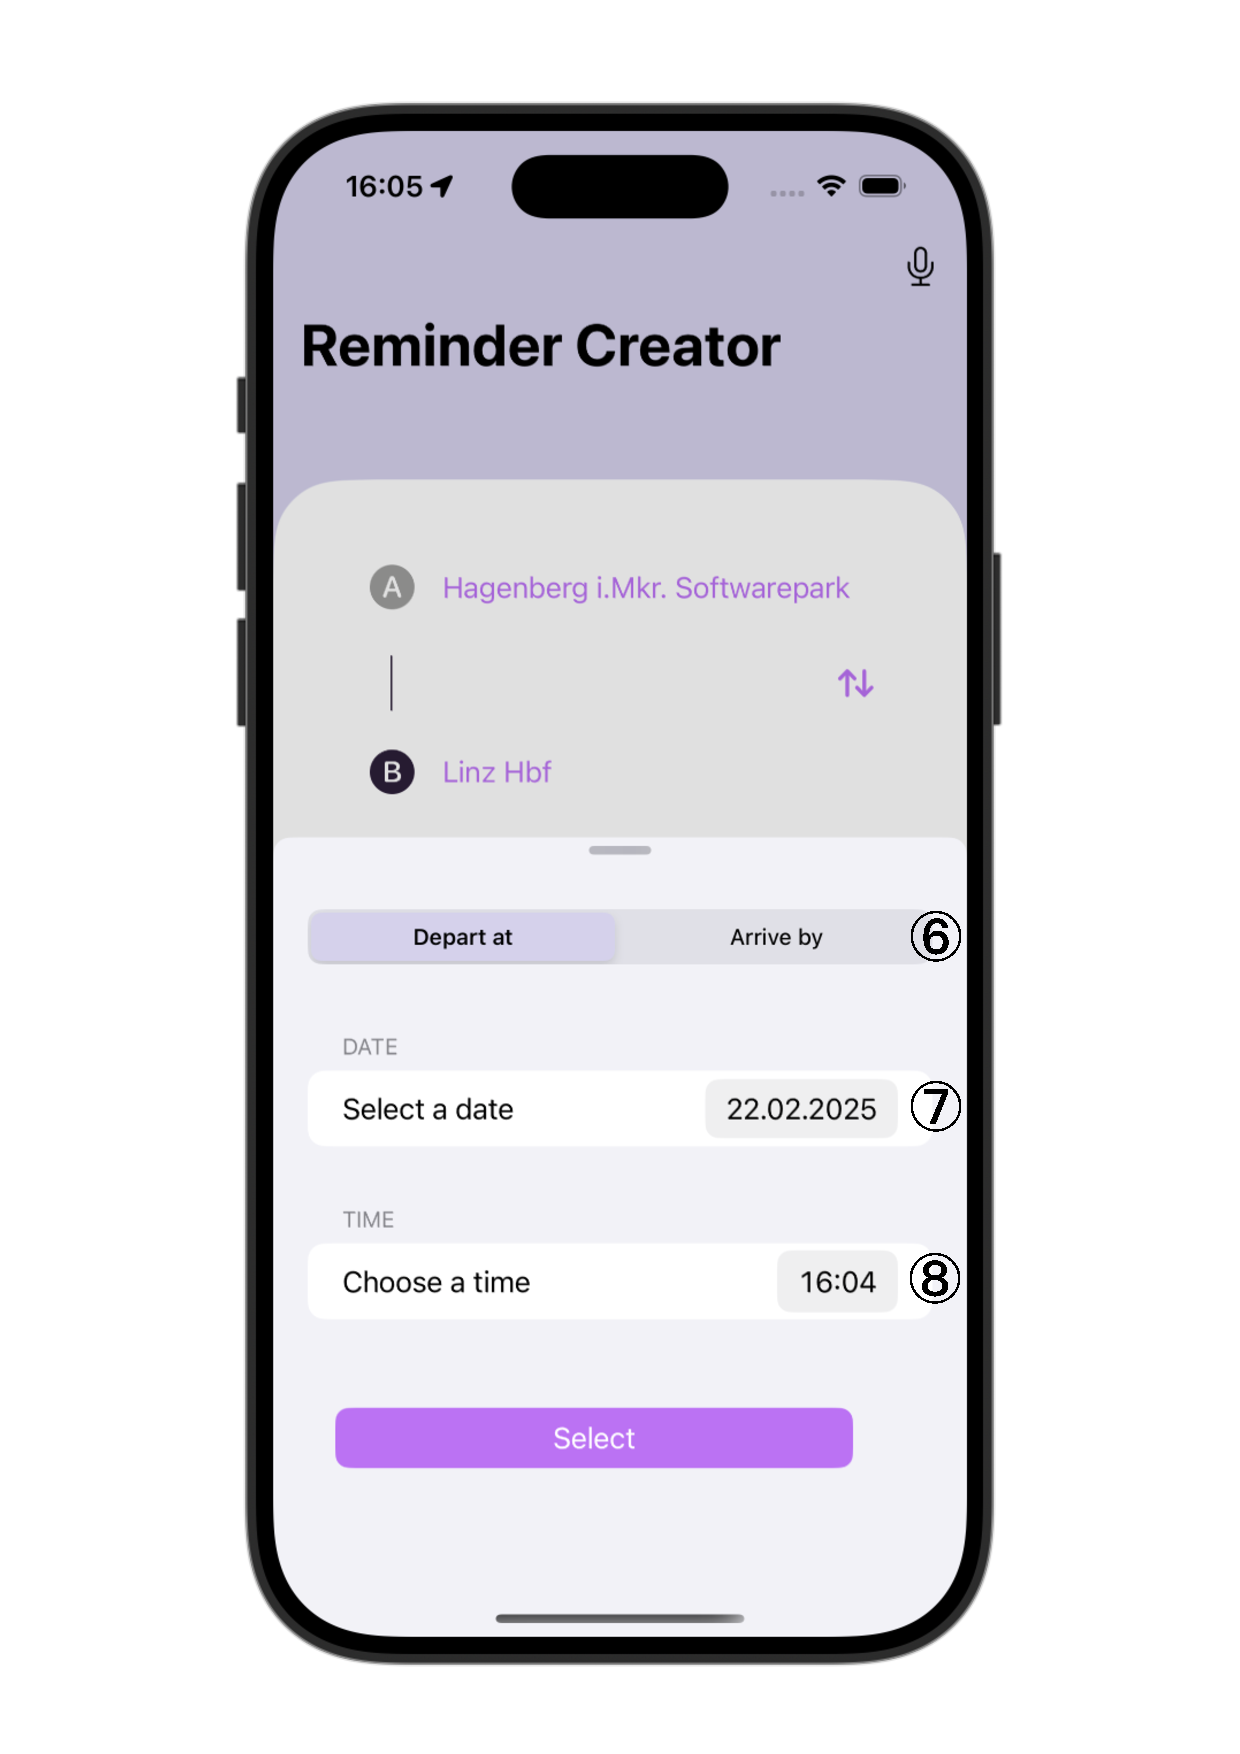
\includegraphics[width=4cm]{CreatorView3.pdf}}}%
    \caption{\lstinline{CreatorView} guides users through trip planning with the main interface (a), \lstinline{StationView} sheet (b) and \lstinline{DateView} sheet (c)}%
    \label{fig:creatorview}%
\end{figure}

\begin{figure}[H]%
    \centering
    \subfloat[\centering]{{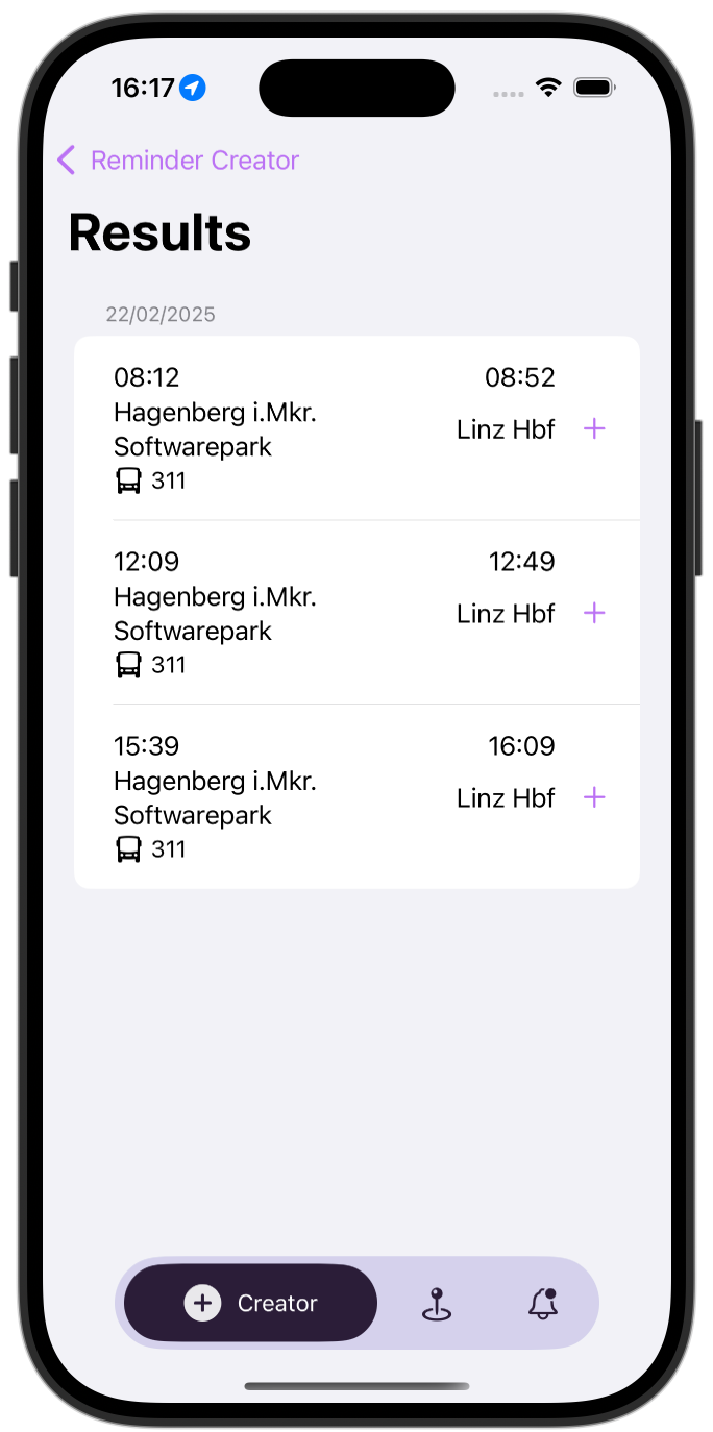
\includegraphics[width=4cm]{CustomizationView.pdf}}}%
    \qquad
    \subfloat[\centering]{{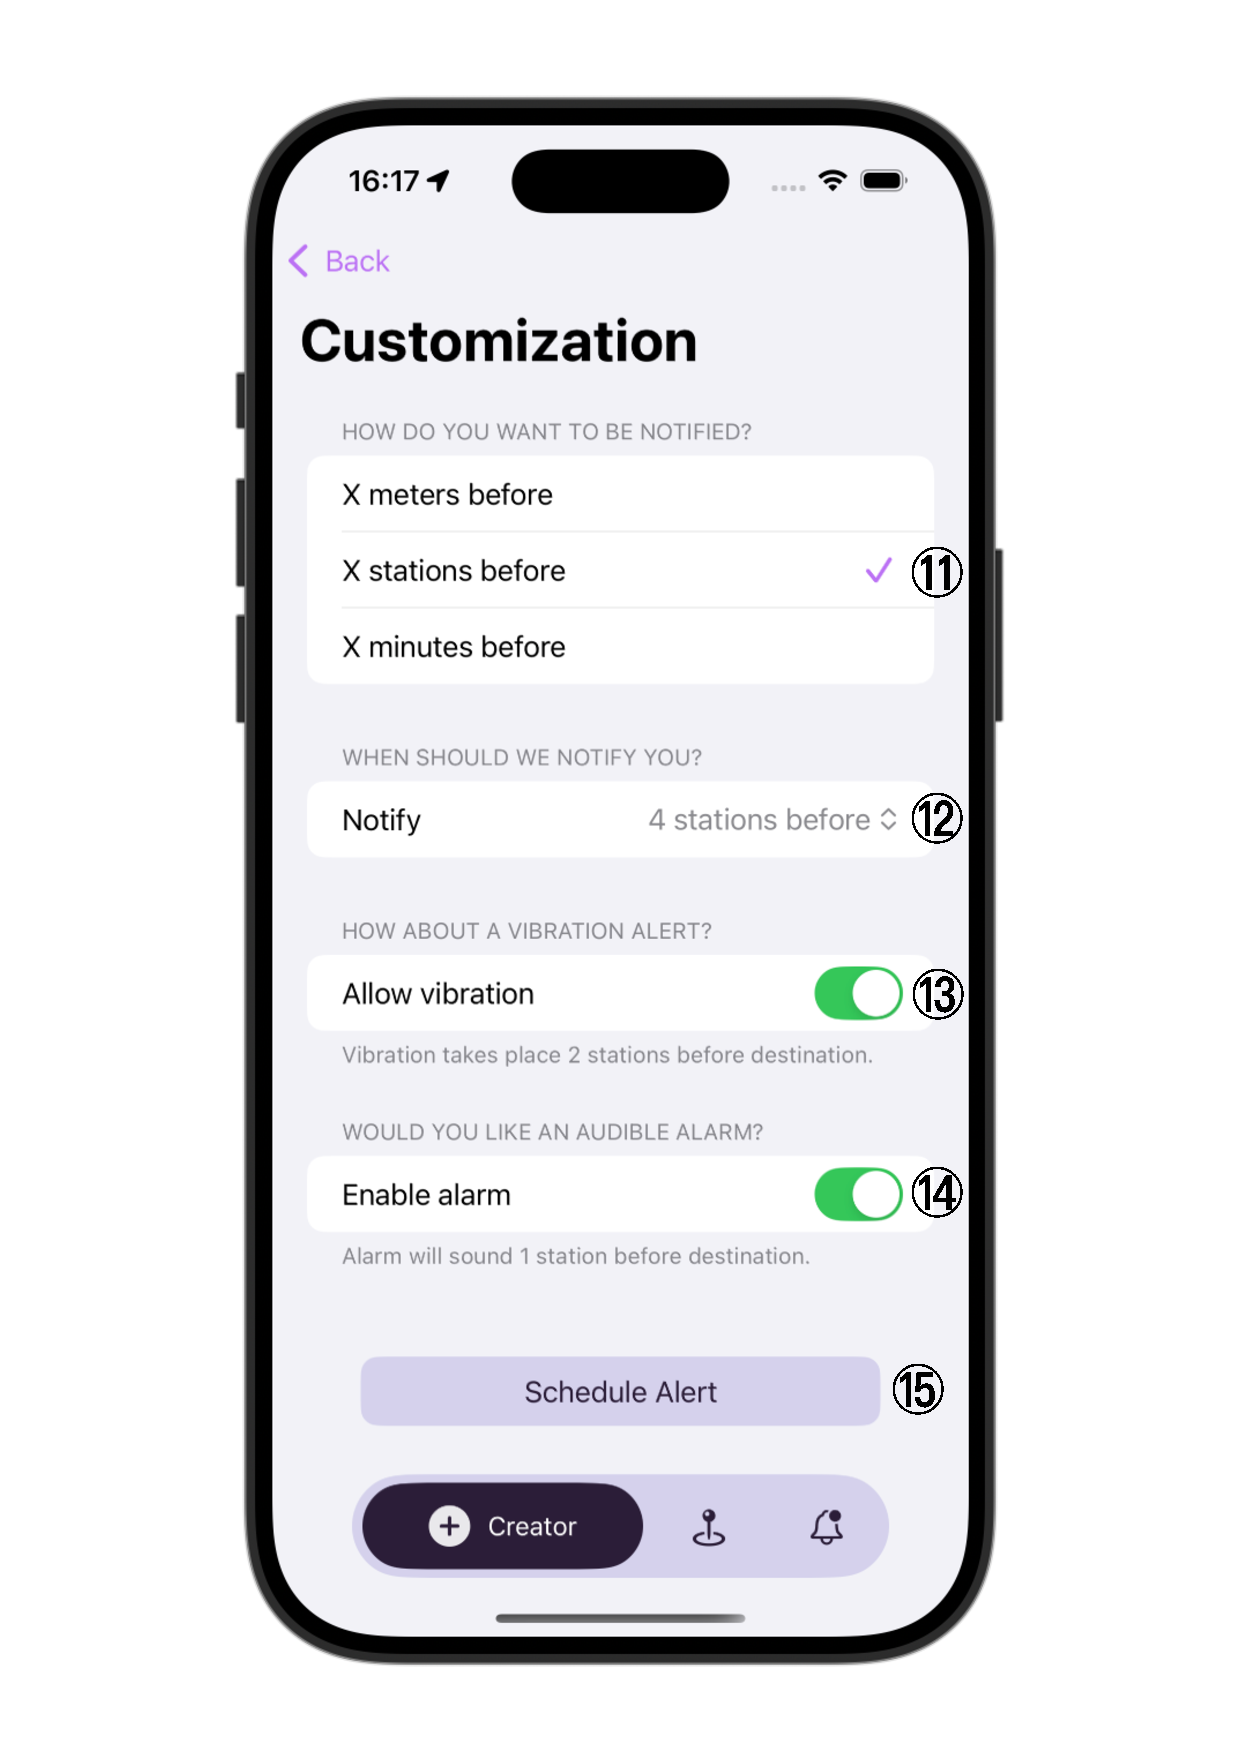
\includegraphics[width=4cm]{CustomizationView2.pdf}}}%
    \caption{\lstinline{ResultView} (a) displays transport connections and \lstinline{CustomizationView} (b) allows users to configure reminder settings}%
    \label{fig:customizationview}%
\end{figure}

\subsection{ReminderView}
The \lstinline{ReminderView} displays all currently scheduled reminders, grouped by date as seen in Figure \ref{fig:reminderview}. 
Each entry \circnum{16} includes the destination name, arrival time, line ID and the interval at which notifications will be sent, and features two buttons: a map icon \circnum{17} and a trash can icon \circnum{18}. 
The map button triggers the system to display the public transportation route on the map and switches to the MapView, the app's third main screen which is discussed in the following section. 
The trash can icon removes the reminder from the database, unschedules the notification and cancels the vibration and alarm if previously enabled.
A plus button \circnum{19} opens the \lstinline{CreatorView}, allowing users to schedule a new reminder.

\begin{figure}[htbp]
    \centering
    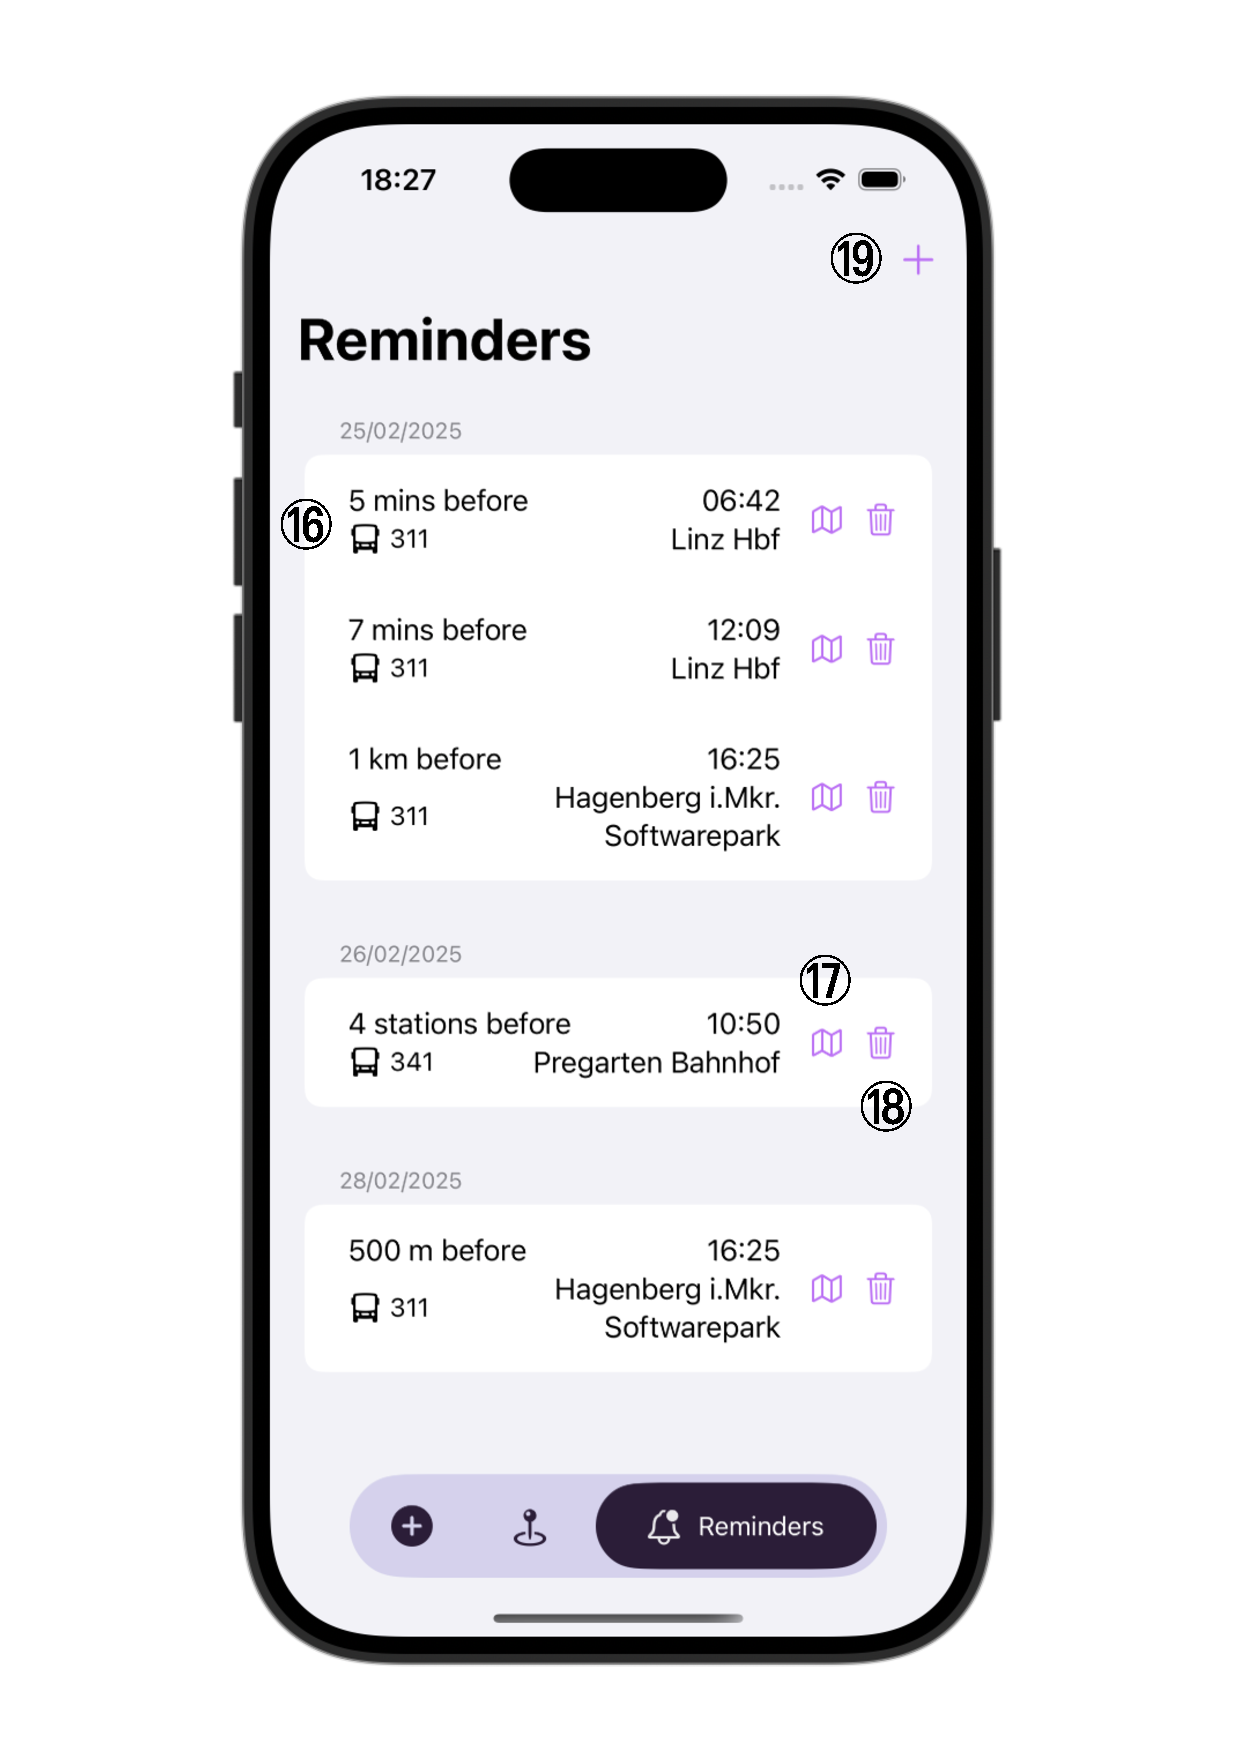
\includegraphics[width=0.35\textwidth]{ReminderView.pdf}
    \caption{\lstinline{ReminderView} displays scheduled reminders with options to view routes on the map or delete entries}
    \label{fig:reminderview}
\end{figure}

\subsection{MapView}
The \lstinline{MapView} displays the user's location and the selected public transportation route on a map. 
Depending on the chosen reminder mode, visual indicators are added to represent when alerts will be triggered. 
If the reminder is based on distance, circles (radii) \circnum{20} are drawn around the destination to indicate the alert zones. 
If it is based on the number of stops, the intermediate stations \circnum{21} where alerts will occur are marked. 
However, for time-based reminders, no visual representation is provided in the app.
Figure \ref{fig:mapview} illustrates these visualizations: (a) represents the radii, (b) highlights the intermediate stops and (c) displays the standard route.
The map icon button \circnum{22} toggles the map layout to satellite view, while the cursor icon button \circnum{23} zooms into the user's current location.

\begin{figure}[htbp]%
    \centering
    \subfloat[\centering]{{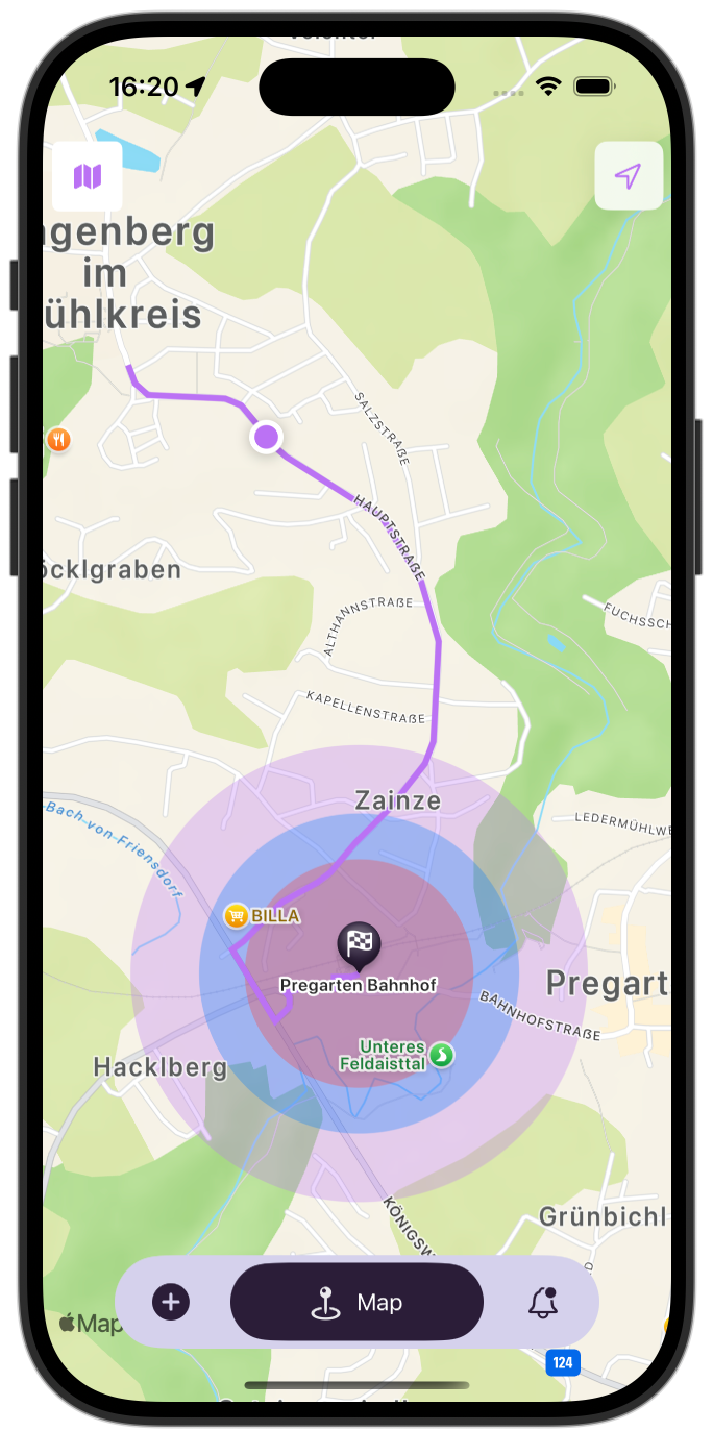
\includegraphics[width=4cm]{MapView.pdf}}}%
    \qquad
    \subfloat[\centering]{{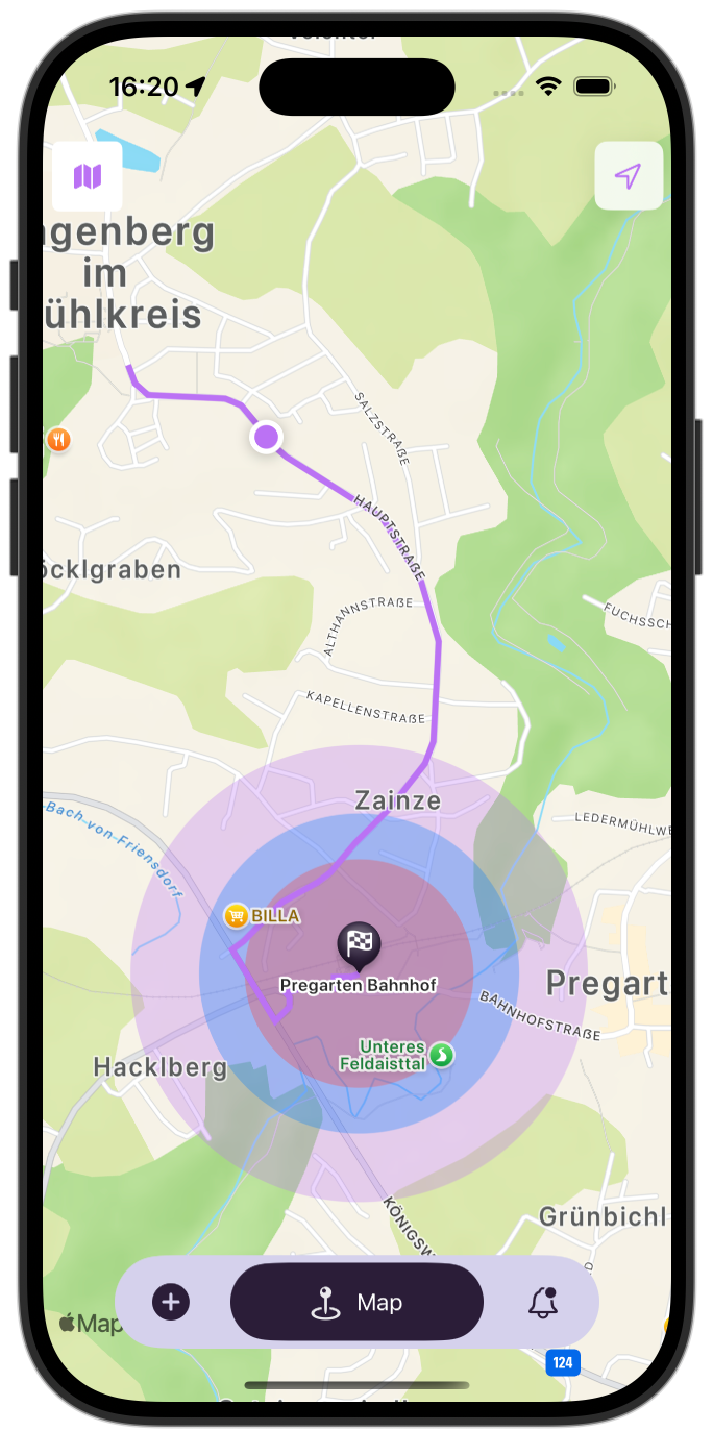
\includegraphics[width=4cm]{MapView.pdf}}}%
    \qquad
    \subfloat[\centering]{{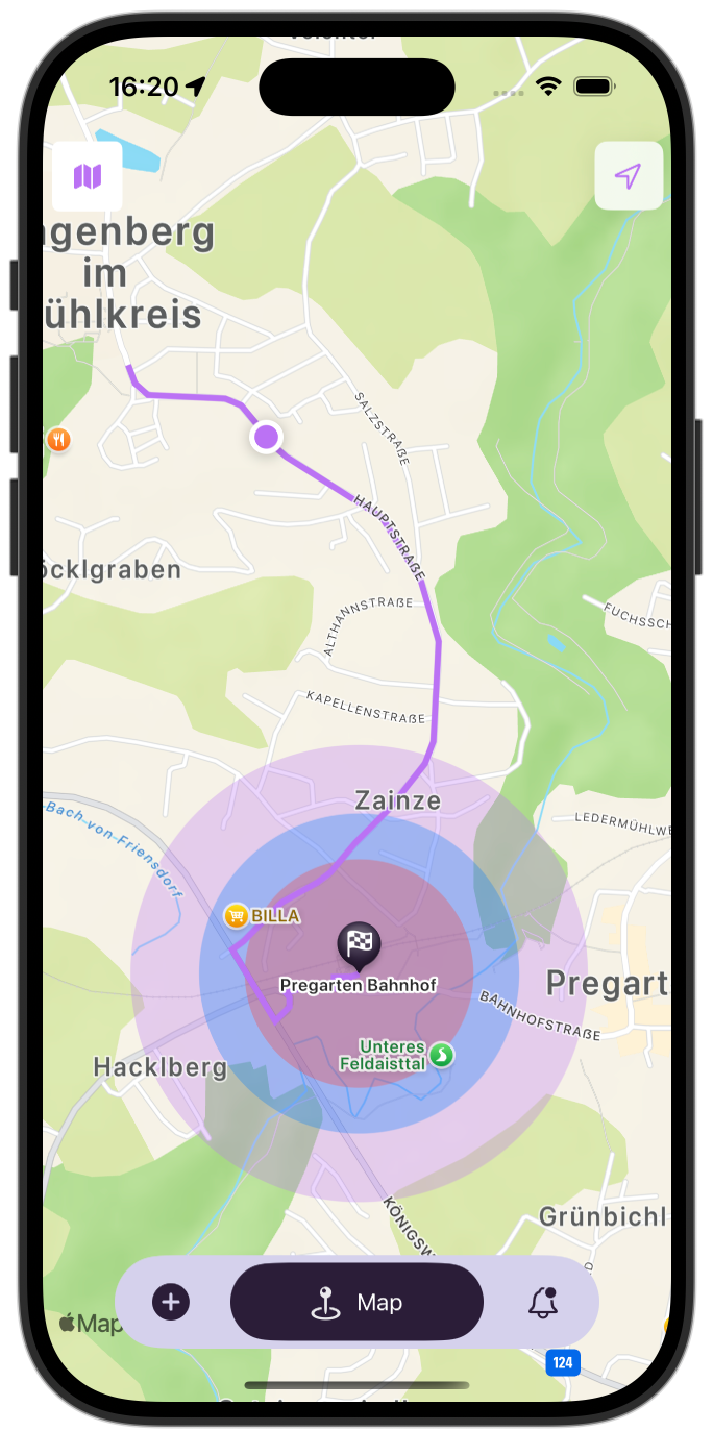
\includegraphics[width=4cm]{MapView.pdf}}}%
    \caption{\lstinline{MapView} displays routes for connections with active reminders showing alert radii (a), intermediate stops (b) or the standard route (c)}
    \label{fig:mapview}%
\end{figure}

\subsection{SpeechRecognitionView}
\label{sec:speechview}
The \lstinline{SpeechRecognitionView} implements a wizard-based approach for setting up reminders through voice input processing. 
The user's speech is transcribed and sent to an AI model along with a structured prompt, which interprets the input and determines the necessary reminder details.
This feature is primarily an experimental implementation intended for exploring how the reminder setup process can be made more accessible and user-friendly for a broader audience. 
It is not a fully developed feature but serves as a prototype for usability testing, further discussed in Section \ref{sec:speech}.

The process is structured into four consecutive views, each prompting the user with a specific question to progressively gather the required details for scheduling a reminder.
However, all views follow the same workflow as illustrated in Figure \ref{fig:speechrecognitionview}.
In the top-right corner, a microphone button \circnum{24} allows the user to start and stop the transcription process. 
Below, an options section \circnum{25} presents the user with three predefined choices as possible answers to the current question. 
As the user speaks, the input is processed and refined to improve accuracy before the transcript is displayed as seen in \circnum{26}.

Once the transcript is available, the user can take further actions using the three buttons at the bottom of the screen. 
Pressing \circnum{27} resets the transcript, allowing the user to reattempt the input. 
Pressing \circnum{28} sends the transcript along with the structured prompt to the AI model, which analyzes the response and attempts to match it to one of the predefined options. 
The selected option is then displayed in \circnum{30}. 
Finally, pressing \circnum{29} checks whether an AI response has been successfully received. 
If so, the system navigates to the next step in the wizard-based flow, progressively collecting all the necessary details until the last view, where the reminders are scheduled.

\begin{figure}[htbp]
    \centering
    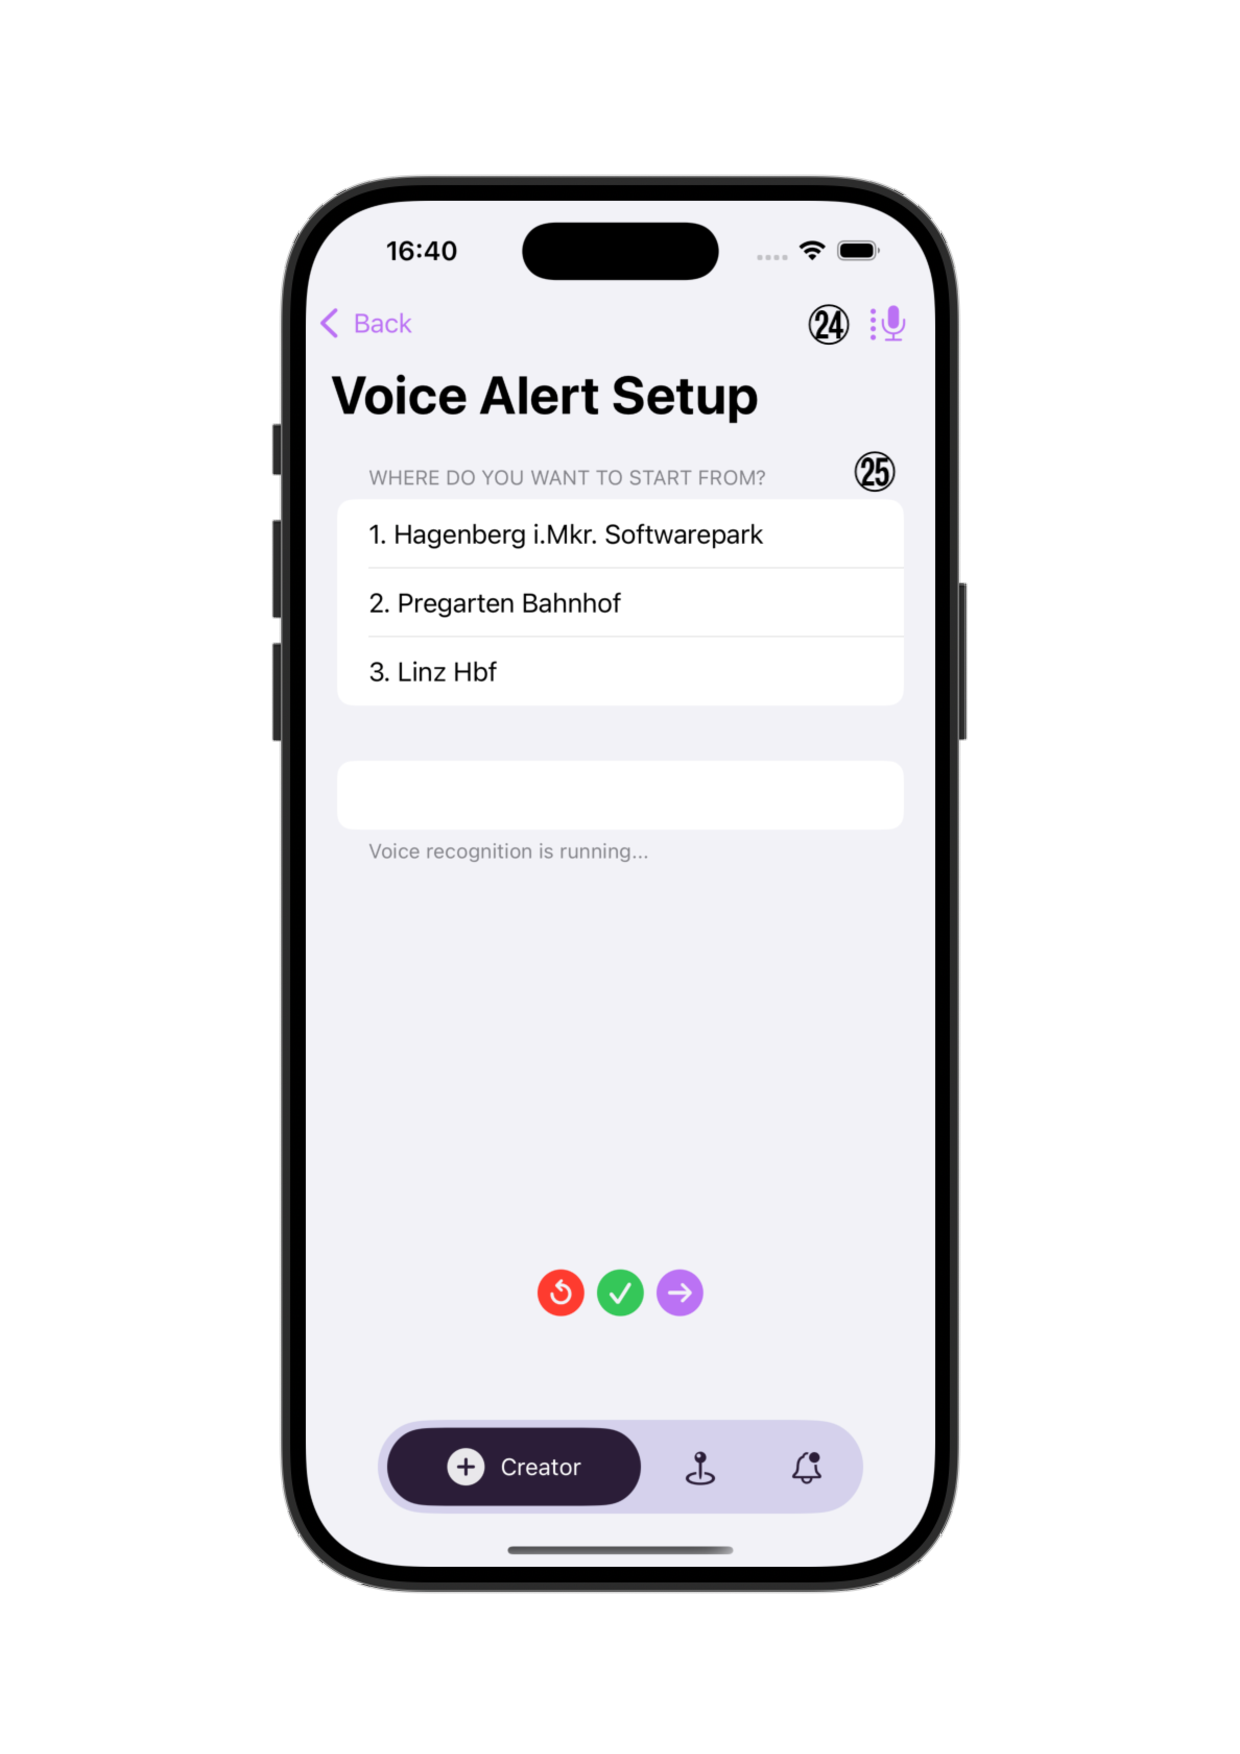
\includegraphics[width=4cm]{SpeechRecognitionView.pdf}
    \qquad
    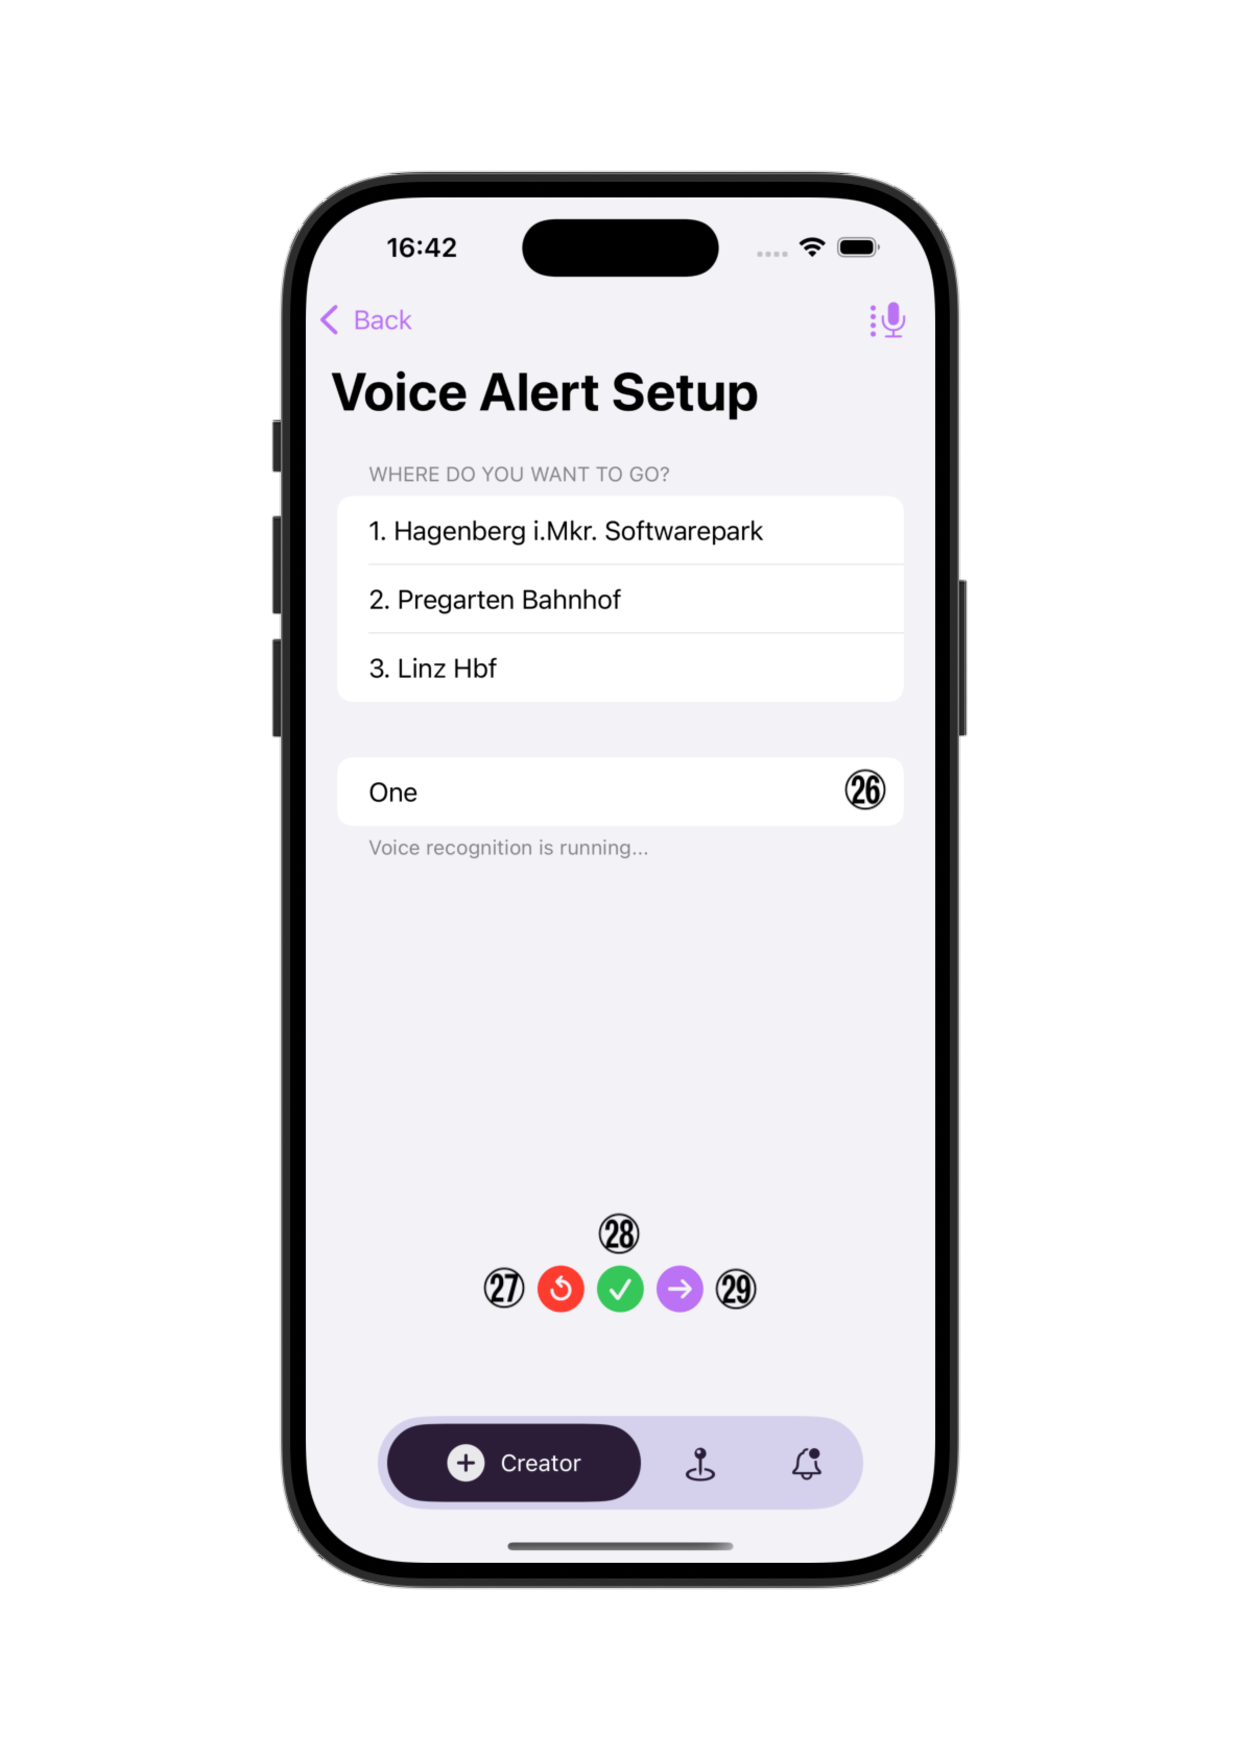
\includegraphics[width=4cm]{SpeechRecognitionView2.pdf}
    \qquad
    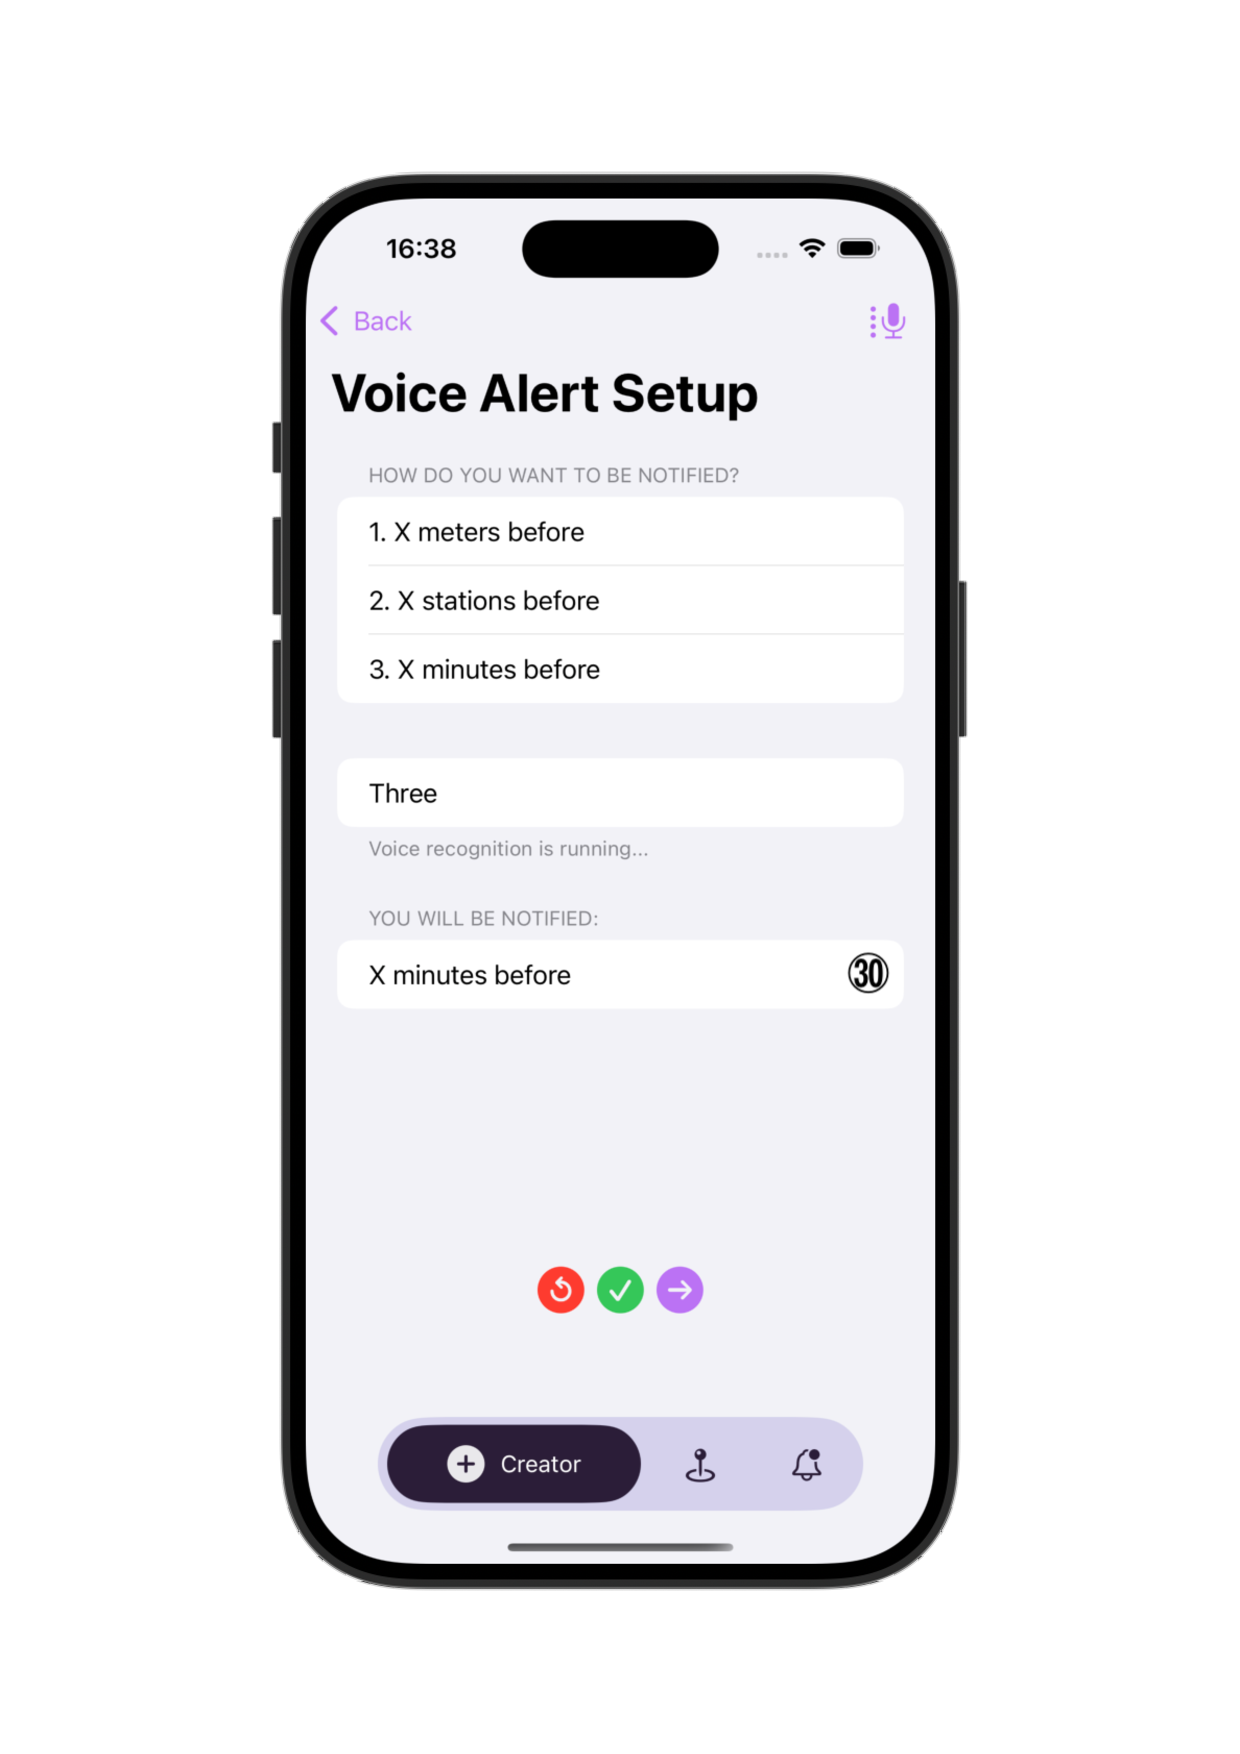
\includegraphics[width=4cm]{SpeechRecognitionView3.pdf}
    \caption{\lstinline{SpeechRecognitionView} guides the user through AI-assisted voice processing for reminder setup}
    \label{fig:speechrecognitionview}
\end{figure}


\section{Reminder Behaviour}
The app triggers reminders such as notifications, vibrations and alarms when users enter predefined geographic zones.
This is handled by a custom \lstinline{LocationManager} class, which extends Apple's \lstinline{CLLocationManager} and follows a singleton pattern to prevent redundant tracking.
The following subsections outline how regions are monitored and alerts are triggered in iOS.

\subsection{Geofencing Methods}
The geofencing process consists of monitoring regions and detecting user entry.
Figure \ref{fig:flow} provides an overview of this process in a flowchart.

\begin{figure}[H]
    \centering
    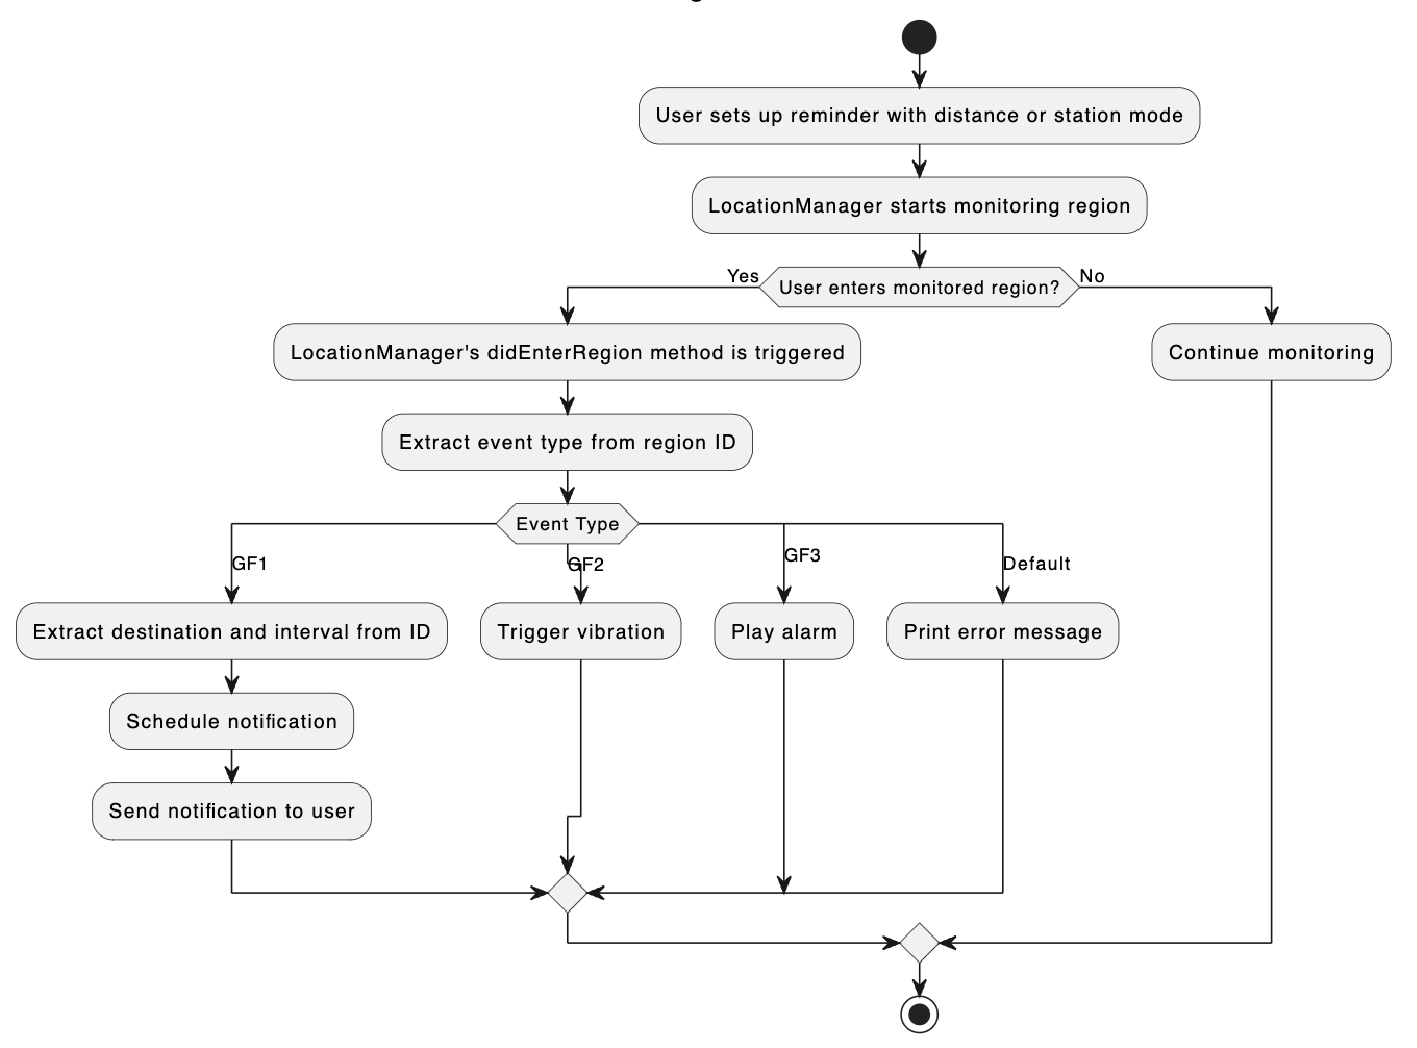
\includegraphics[width=0.99\textwidth]{Flowchart.pdf}
    \caption{Flowchart illustrating the geofencing process}
    \label{fig:flow}
\end{figure}

\subsubsection{Start Monitoring}
The function in Program \ref{prog:startmonitoring} demonstrates how a geofence is created and registered for monitoring.
Before creating the geofence, the function first checks whether geofencing is supported on the device. 
This ensures that the app does not attempt to monitor geofences on unsupported hardware. 
If monitoring is available, a \lstinline{CLCircularRegion} object is created using a central coordinate (latitude and longitude), a radius that determines its size and a unique identifier. 
The properties \lstinline{notifyOnEntry} and \lstinline{notifyOnExit} determine whether notifications are triggered when the user enters or exits the region. 
In this app, only entry notifications are relevant, meaning \lstinline{notifyOnEntry} is set to true, while \lstinline{notifyOnExit} remains false.
Once the \lstinline{CLCircularRegion} is configured, the function registers the geofence with the system.

\begin{program}[htbp]
\begin{SwiftCode}
let locationManager = CLLocationManager()
func startMonitorRegionAtLocation(center: CLLocationCoordinate2D, radius: Double, identifier: String) {
    if CLLocationManager.isMonitoringAvailable(for: CLCircularRegion.self) {
        let region = CLCircularRegion(center: center, radius: radius, identifier: identifier)
        region.notifyOnEntry = true
        region.notifyOnExit = false
        locationManager.startMonitoring(for: region)
    }
}\end{SwiftCode}
\caption{Function for starting region monitoring}
\label{prog:startmonitoring}
\end{program}

\subsubsection{Stop Monitoring}
To stop monitoring a geofenced region, the function takes the identifier of the region as a parameter. 
The \lstinline{CLLocationManager} maintains a list of currently monitored regions, which can be accessed through its monitoredRegions property. 
Using this, the function searches for a geofence that matches the given identifier. 
If a corresponding region is found, monitoring is stopped as shown in Program \ref{prog:stopmonitoring}.

\begin{program}[htbp]
\begin{SwiftCode}
func stopMonitorRegionAtLocation(identifier: String) {
    if let region = manager.monitoredRegions.first(where: {$0.identifier == identifier}) {
        manager.stopMonitoring(for: region)
    }
}\end{SwiftCode}
\caption{Function for stopping region monitoring}
\label{prog:stopmonitoring}
\end{program}

\subsubsection{Region Entry}
In order to trigger an action based on a user entering a monitored region, the \lstinline{CLLocationManager} provides the delegate method \lstinline{didEnterRegion}, which is automatically called when a user enters a geofenced area. 
However, this method does not allow for additional parameters to be passed, meaning that only the region object is available within the function.
To ensure the correct action is taken upon entering a geofenced area, the app must differentiate between different geofencing levels, each corresponding to a different type of alert. 
To achieve this, the simplest approach is string concatenation, where a \ac{UUID} is combined with a prefix that indicates the type of geofence. 
In this implementation, the following naming convention is used: GF1 represents Geofence Level 1 which triggers a notification, GF2 for a vibration and GF3 for an alarm.
For notifications, the identifier string also includes the destination name and the reminder interval, which are extracted to generate the notification content. 
Program \ref{prog:didenterregion} demonstrates how the \lstinline{didEnterRegion} function processes a geofence entry event and triggers the corresponding action.

\begin{program}[htbp]
\begin{SwiftCode}
func locationManager(_ manager: CLLocationManager, didEnterRegion region: CLRegion){
    guard let eventType = extractEventType(from: region.identifier) else {return}
    switch eventType {
    case "GF1":
        if let idInfo: [String] = extractIdInfoForNotification(using: region.identifier) {
            scheduleNotification(destination: idInfo[0], interval: idInfo[1], id: idInfo[2])}
    case "GF2": vibrate()
    case "GF3": playAlarm()
    default: print("Unknown event type: \(eventType)")
    }
}\end{SwiftCode}
\caption{Function for handling monitored region entry events}
\label{prog:didenterregion}
\end{program}

\subsection{Triggered Actions}
When a monitored region is entered, a geofence event triggers predefined actions. 
These actions include sending notifications, triggering vibration feedback and playing an audible alarm.
These alerts ensure that users are notified in time for their stop. 
In contrast, the time-based mode schedules these actions for a specific time and date, independent of location.
The following subsections detail the implementation of these triggered actions in SwiftUI.

\subsubsection{Notification}
Notifications serve as a subtle first reminder to users as they approach their destination. 
The \lstinline{scheduleNotification} function in Program \ref{prog:notification} creates a notification request using \lstinline{UNUserNotificationCenter}.
The \lstinline{UNMutableNotificationContent} object is populated with a title containing the reminder interval and a body displaying the final destination. 
To ensure the notification is noticeable, a critical sound alert is enabled using \lstinline{UNNotificationSound.defaultCritical}. 
The notification trigger is set to fire after a one-second delay, ensuring immediate execution when the function is called.

To allow cancellation of a previously scheduled notification, the \lstinline{cancelNotification} function removes pending notification requests associated with a given identifier. 
This ensures that users do not receive outdated alerts if their travel plans change.
Figure \ref{fig:notification} illustrates how a received notification appears within the app.

\begin{figure}[htbp]
    \centering
    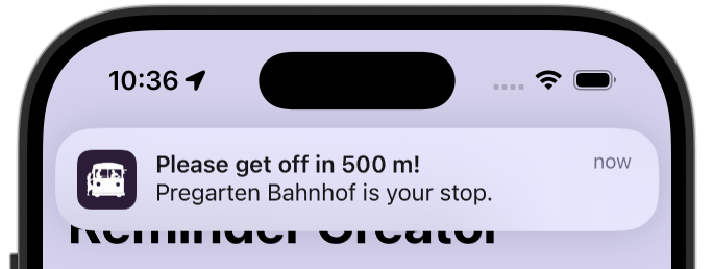
\includegraphics[width=0.55\textwidth]{Notification.pdf}
    \caption{Notification alerting the user about their stop}
    \label{fig:notification}
\end{figure}

\begin{program}[htbp]
\begin{SwiftCode}
func scheduleNotification(destination: String, interval: String, id: String) {
    let content = UNMutableNotificationContent()
    content.title = "Please get off \(interval)!"
    content.body = "\(destination) is your stop."
    content.sound = UNNotificationSound.defaultCritical
    let trigger = UNTimeIntervalNotificationTrigger(timeInterval: 1, repeats: false)
    let request = UNNotificationRequest(identifier: id, content: content, trigger: trigger)
    UNUserNotificationCenter.current().add(request) { error in
        print(String(describing: error?.localizedDescription))
    }
}
func cancelNotification(for id: String) {
    UNUserNotificationCenter.current().removePendingNotificationRequests(withIdentifiers: [id])
}\end{SwiftCode}
\caption{Triggering and canceling a local notification}
\label{prog:notification}
\end{program}

For the time-based mode, the notification must be scheduled to fire at an exact time.
Instead of an immediate trigger, the app constructs a \lstinline{UNCalendarNotificationTrigger} using an instance of \lstinline{DateComponents}, as seen in Program \ref{prog:notification2}. 
Although the trigger type differs, the rest of the notification setup including the content configuration and request creation remains the same.

\begin{program}[htbp]
\begin{SwiftCode}
let trigger = UNCalendarNotificationTrigger(dateMatching: dateComponents, repeats: false)\end{SwiftCode}
\caption{Scheduling a local notification at a specific time}
\label{prog:notification2}
\end{program}

\subsubsection{Vibration}
Vibration feedback serves as a more noticeable second reminder to the user.
The function shown in Program \ref{prog:vibration} utilizes the AVFAudio framework to initiate a short vibration pulse.

\begin{program}[htbp]
\begin{SwiftCode}
@objc func vibrate() {
    AudioServicesPlayAlertSound(kSystemSoundID_Vibrate)
}\end{SwiftCode}
\caption{Triggering a vibration}
\label{prog:vibration}
\end{program}

For the time-based mode, a \lstinline{Timer} object is used instead of a geofence event to trigger the vibration at a designated time as described in Program \ref{prog:vibration2}. 
The \lstinline{Timer} object is initialized with an instance of \lstinline{DateComponents} and once the time arrives, the \lstinline{Timer} executes the function.
The vibrate function in Program \ref{prog:vibration} is marked with \texttt{@objc} because it is referenced by \texttt{\#selector} in the \lstinline{Timer} object initialization. 
In Swift, methods used as selectors must be exposed to Objective-C runtime. 
Without \texttt{@objc}, the Swift compiler would not be able to locate the function at runtime when triggered by the \lstinline{Timer} class.

To allow for cancellation of a previously scheduled vibration, \lstinline{RunLoop.main.cancelPerform} is used. 
This method ensures that if a scheduled vibration is no longer needed, such as when a reminder is canceled, the function call is removed from the execution queue.

\begin{program}[htbp]
\begin{SwiftCode}
let timer = Timer(fireAt: dateComponents, interval: 0, target: self, selector: #selector(vibrate), userInfo: reminder.id, repeats: false)
RunLoop.main.add(timer, forMode: .common)
RunLoop.main.cancelPerform(#selector(vibrate), target: self, argument: id)\end{SwiftCode}
\caption{Scheduling and canceling a vibration at a specific time}
\label{prog:vibration2}
\end{program}

\subsubsection{Alarm}
The audible alarm acts as a last-resort alert to ensure the user is fully aware that they need to get off.
Unlike notifications and vibrations, the alarm is highly intrusive making it difficult to miss.
The function presented in Program \ref{prog:alarm} uses the \lstinline{AVAudioPlayer} class from the AVFAudio framework to play a MP3 sound file. 
The function retrieves the file from the app bundle and initializes the audio player. 
If the file is missing or the initialization fails, an error is printed to aid debugging.
For the time-based mode, the alarm can be scheduled and canceled just like in Program \ref{prog:vibration2} by switching the selector to \texttt{\#selector(playAlarm)}.

\begin{program}[htbp]
\begin{SwiftCode}
@objc func playAlarm() {
    var audioPlayer: AVAudioPlayer?
    let soundFileName = "alert_extreme.mp3"
    guard let soundURL = Bundle.main.url(forResource: soundFileName, withExtension: nil) else {
        fatalError("Unable to find \(soundFileName) in bundle")
    }
    do {
        audioPlayer = try AVAudioPlayer(contentsOf: soundURL)
    } catch {
        print(error.localizedDescription)
    }
    audioPlayer?.play()
}\end{SwiftCode}
\caption{Triggering an alarm}
\label{prog:alarm}
\end{program}

\section{Improving User Experience of App}
\label{sec:speech}
To make the reminder setup more user-friendly and intuitive, two approaches have been tested and combined into a test feature in the app. 
The first approach is a step-by-step wizard, which guides users through the setup in a structured way.
The second allows users to set reminders using speech input.
The sequence diagram in Figure \ref{fig:sequence} breaks down how the system components interact during speech-based input, from recognizing speech and processing it with AI to displaying the recognized option and finally scheduling the reminder.
Testing has shown that while speech input has potential, Apple's Speech framework struggles with consistently accurate transcriptions. 
This limitation is one of the reasons why the wizard-based approach was explored as well, as it reduces the need for free-form input and instead guides users through predefined choices.

\begin{figure}[htbp]
    \centering
    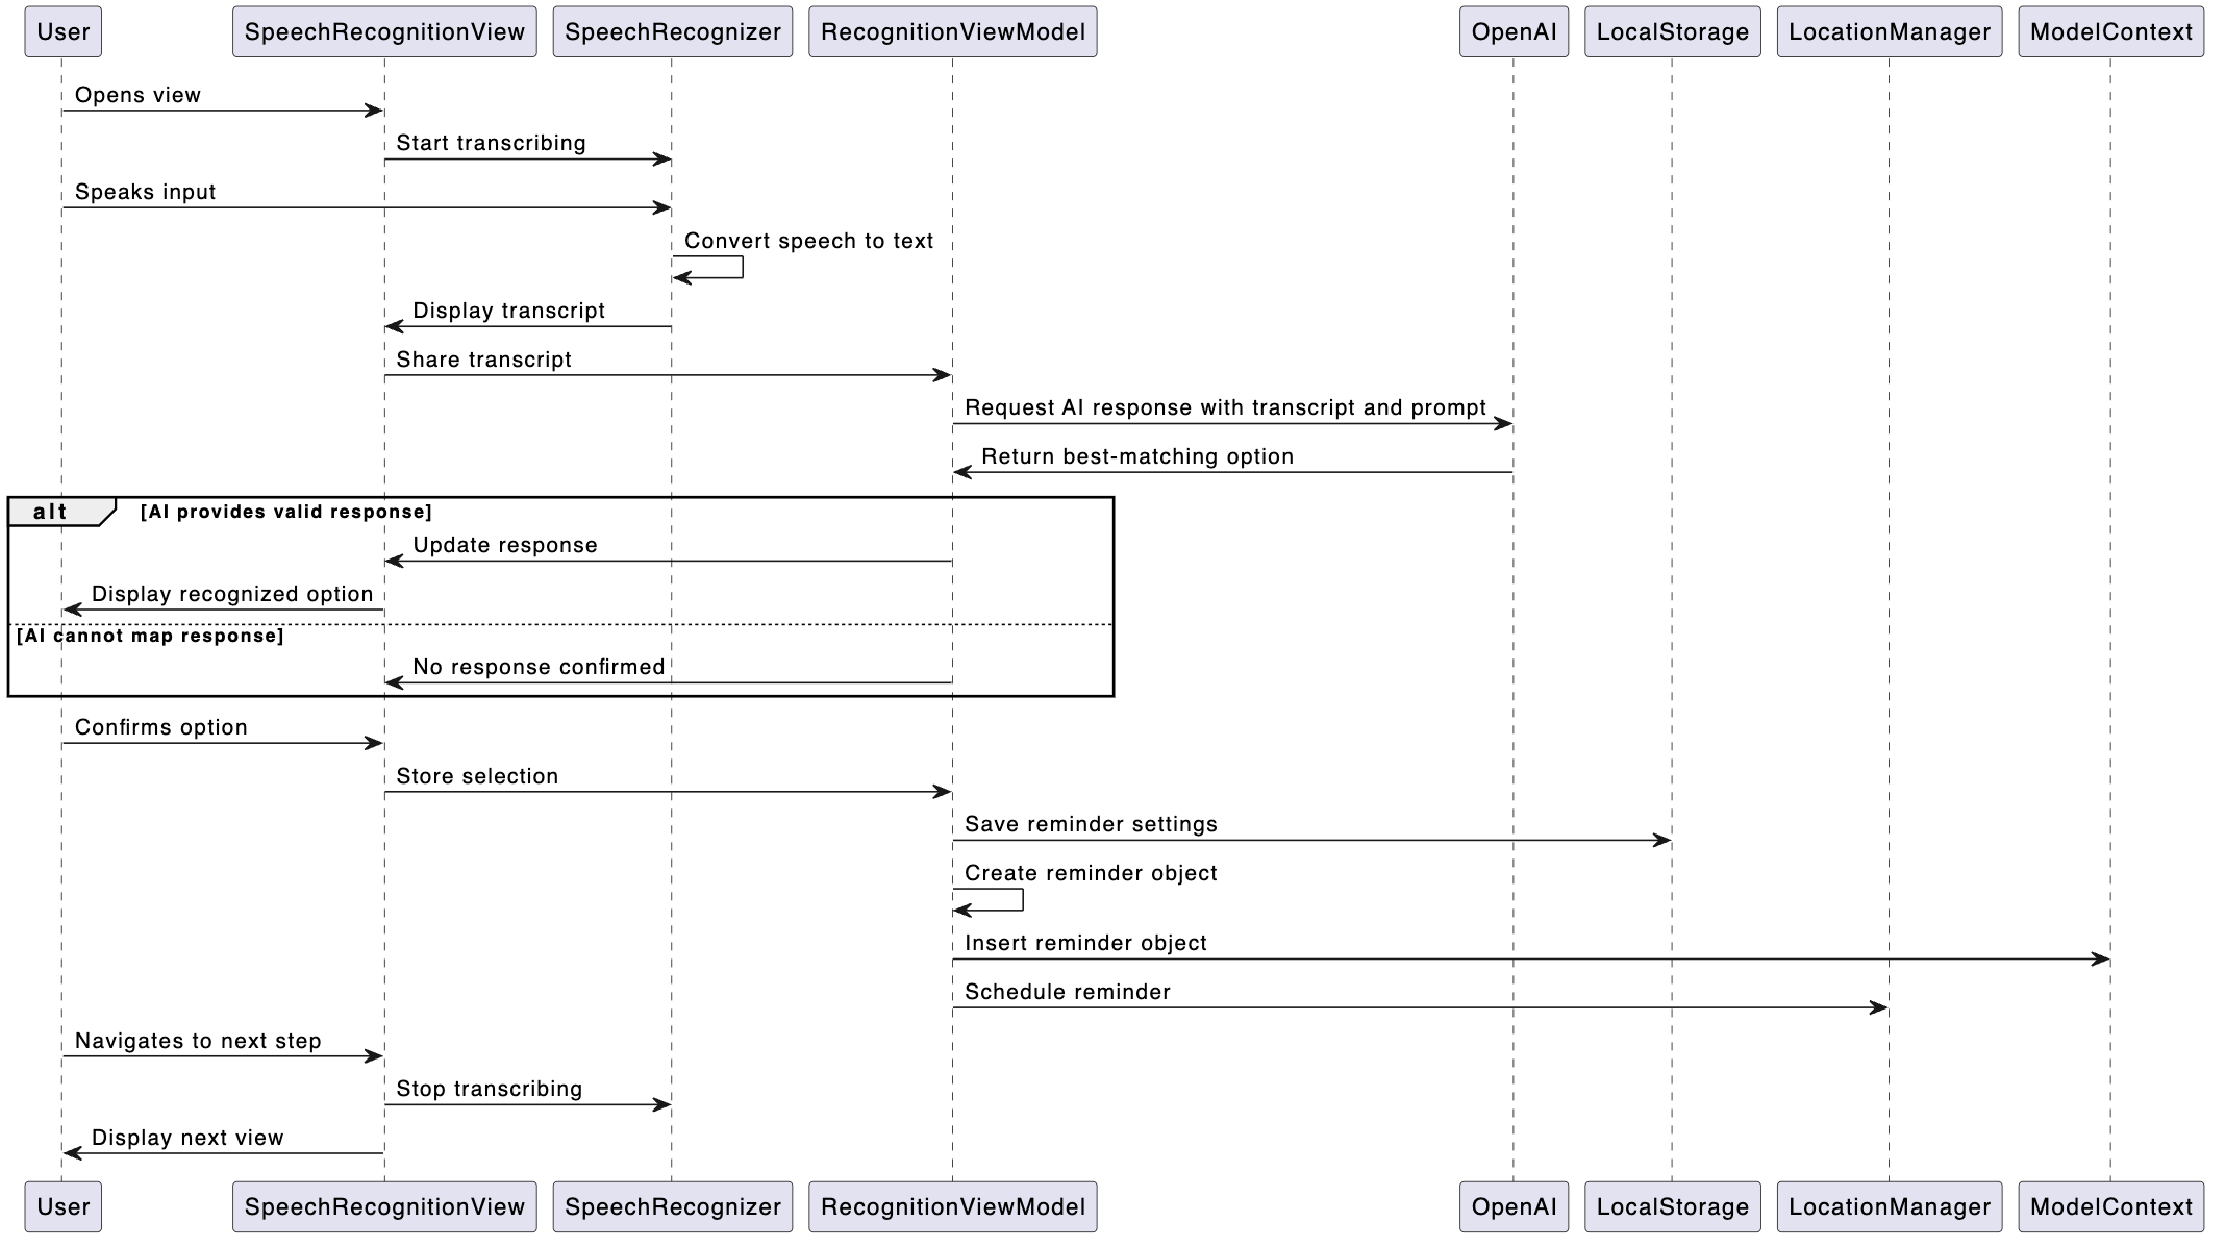
\includegraphics[width=0.99\textwidth]{SequenceDiagram.pdf}
    \caption{Sequence diagram for the voice-controlled reminder setup}
    \label{fig:sequence}
\end{figure}